%%%%%%%%%%%%%%%%%%%%%%%%%%%%%%%%%%%%%%%%%%%
\subsection{Grey Level Co-Occurence Matrix}
%%%%%%%%%%%%%%%%%%%%%%%%%%%%%%%%%%%%%%%%%%%
A Grey Level Co-Occurrence Matrix (GLCM) is able to quantify the spatial frequency distribution of grey level pixel intensity pairs. The GLCM matrix is formed by determining the frequency of grey level value pixel pairs for a given image.  A relationship is set a priori to determine the direction for grey level comparison.  This relationship is an angle relating a pixel to its neighbor, and is chosen in multiples of either 0 or 45 degrees.  Common GLCM spatial relationships are $0, \pi/4, 3\pi/4$, and $\pi/2$ radians.
%
\begin{figure}[!htb]
    \begin{center}
        \makebox[\textwidth]{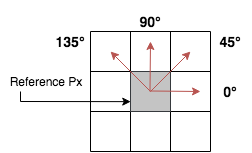
\includegraphics[scale=0.75]{/Sources/Background/Texture_and_Tone/glcm-relationships-no-title.png}}
    \end{center}
    \caption{Defining GLCM Relationships}
    \label{fig:texture}
\end{figure}
%
In order to quantify a texture in a rotationally consistent fashion, all four relationships are usually calculated and averaged together in determining the overall GLCM matrix.  The GLCM has a size of $N x N$ where $N$ is the discrete quantized levels.

A single relationship Co-Occurence matrix is formulated such that,
%
\begin{align}
    \mathbf{\phi}_{ij}(\triangle x,\triangle y) = \sum_{x=0}^{n}\sum_{y=0}^{m}
    \begin{cases}
        1, if I(x,y) = i \quad \textrm{and} \quad  I(x+\triangle x,y+\triangle y) = j \\
        0, otherwise
    \end{cases}
\end{align}
%
where $I(x,y)$ is an $n x m$ image and $\triangle x,\triangle y$ represent the predefined offset of the grey level pixel neighbor intensity relationship (i,j).
Being defined as referencing one pixel to its neighbor to the right (0 degrees) the GLCM matrix is formulated as such,
%
\begin{figure}[!htb]
    \begin{center}
        \makebox[\textwidth]{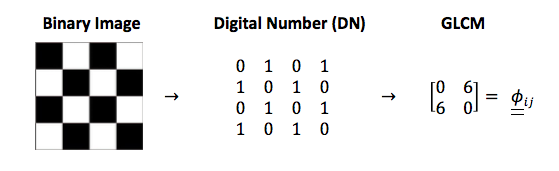
\includegraphics[scale=0.75]{/Sources/Background/Texture_and_Tone/glcm.png}}
    \end{center}
    \caption{Converting a Binary Image to a GLCM Matrix}
    \label{fig:texture}
\end{figure}
The example in Figure 2.12 shows the simplest case of a binary image, or an image that only contains white and black pixels.  These pixels values captured by a camera are then converted into there corresponding digital numbers, in this case either zero or one.  With the spatial relationship being defined as one to the right, the GLCM matrix is then formed.

Non symmetrical GLCMs should be symmetrized by adding each to its transpose,
%
\begin{align}
    \mathbf{\phi}^{'} = \mathbf{\phi} + \mathbf{\phi}^{T}
\end{align}
%
Normalizing the frequency to one by dividing the matrix by the sum of all its elements, results in a probability distribution for each grey level pixel pair.
%
\begin{align}
    \mathbf{P} = \frac{\mathbf{\phi}^{'}}{\sum_{i=0}^{N-1}\sum_{j=0}^{N-1}\mathbf{\phi}^{'}}
\end{align}
%
where for the example given above the resulting $\mathbf{P}$ is
%
\begin{align}
    \mathbf{P} = \frac{1}{12}
    \begin{bmatrix}
        0 & 6 \\
        6 & 0
    \end{bmatrix}
    =
    \begin{bmatrix}
        0 & 0.5 \\
        0.5 & 0
    \end{bmatrix}
\end{align}
%
As expected the probability of finding a 0 next to a 1 is the same as finding a 1 next to a zero in a binary checkerboard image.

Features can then be extracted from the formed matrix for the purpose of defining single quantitative values for texture.  These features are known as Haralick features and generally fall into 3 distinct feature categories; Contrast, Statistical and measures of Orderliness \cite{calgary}.

Contrast measures are defined by weights that increase or decrease with distance from the GLCM diagonal.  These weights can be linear, exponential, etc. For the N x N dimensional GLCM matrix the N - 1 term in the first row or column represents pixel relationships that are of the greatest intensity difference.

For example, an 8-bit image has 256 possible grey level values ranging from 0-255, so the maximum amount of contrast occurs when pixel pairs (i,j) are either (0, 255) or (255, 0).

Contrast has weights that increase exponentially away from the diagonal.  It is calculated as
%
\begin{align}
    Contrast = \sum_{i=0}^{N-1}\sum_{j=0}^{N-1}(i-j)^2P_{ij}
\end{align}
%
The dissimilarity is a measure of contrast with weights that increase linearly away from the diagonal
%
\begin{align}
    Diss = \sum_{i=0}^{N-1}\sum_{j=0}^{N-1}|i-j|P_{ij}
\end{align}
%
The dissimilarity of the example binary image can be calculated as
%
\begin{align}
    Diss = \sum_{i=0}^{N-1}\sum_{j=0}^{N-1}|i-j|P_{ij}
    = \sum_{1=0}^{1}|i|P_{i0}+|i-1|P_{i1}
    = 0 + P_{01} + 0 + P_{10} = \frac{1}{3}
\end{align}
%
Statistical measures utilize each individual element of the GLCM as weights to determine the moments of the probability distribution matrix. The mean, variance, correlation, etc. are not measures of individual pixel intensity values, but rather of the intensity of a pixel in relation to its neighbor’s intensity. The mean is the first central moment and is defined by
%
\begin{align}
    \mu_i = \sum_{i=0}^{N-1}\sum_{j=0}^{N-1}iP_{ij} \\
    \mu_j = \sum_{i=0}^{N-1}\sum_{j=0}^{N-1}jP_{ij}
\end{align}
%
Variance is the second moment of the GLCM and is defined as,
%
\begin{align}
    \sigma_i = \sum_{i=0}^{N-1}\sum_{j=0}^{N-1}(i-\mu_i)^2P_{ij}
\end{align}
\begin{align}
    \sigma_j = \sum_{i=0}^{N-1}\sum_{j=0}^{N-1}(j-\mu_j)^2P_{ij}
\end{align}
%
The correlation shows the “linear dependency of grey level values in the Co-Occurence matrix”\cite{haralickcancer}.  It is computed from the values of the variance and mean such that
%
\begin{align}
    Corr = \sum_{i=0}^{N-1}\sum_{j=0}^{N-1}(\frac{(i-\mu_i)(j-\mu_j)}{\sqrt{\sigma_i^2 \sigma_j^2}})
\end{align}
%
If a the GLCM is symmetric, the x and y means and variances are equal and the equations simplify to,
%
\begin{align}
    \mu = \sum_{i=0}^{N-1}\sum_{j=0}^{N-1}iP_{ij}
\end{align}
\begin{align}
    \sigma = \sum_{i=0}^{N-1}\sum_{j=0}^{N-1}(i-\mu)^2P_{ij}
\end{align}
\begin{align}
    Corr = \sum_{i=0}^{N-1}\sum_{j=0}^{N-1}(\frac{(i-\mu)(j-\mu)}{\sigma^2})
\end{align}
%
Measures of orderliness are quantified by the amount of entropy and energy within an image.  Entropy is a measure of randomness in a system.  In thermodynamics, it is the heat lost when a reaction occurs and hence is a measure of disorder.  Energy is a measure of useful work that can occur due to the non random nature of the energy in a system. (clean up this bit on entropy)

The angular second moment (ASM) describes the amount of “inertia” around a pixel neighbor relationship and is defined as,
%
\begin{align}
    ASM = \sum_{i=0}^{N-1}\sum_{j=0}^{N-1}P_{ij}^2
\end{align}
%
The square root of the ASM results in the energy of the system
%
\begin{align}
    Energy = \sqrt{ASM}
\end{align}
%
For perfectly uniform textures the energy will be at a maximum of 1.
